%%
\documentclass[%
]{ittmm}


\usepackage{polyglossia}
\setdefaultlanguage[spelling=modern]{russian}
\setotherlanguages{english}

%%% One can fix some overfulls
\sloppy

%% Minted listings support
%% Need pygment <http://pygments.org/> <http://pypi.python.org/pypi/Pygments>
\usepackage{minted}
%% auto break lines
\setminted{breaklines=true}

\addbibresource{main.bib}

%% end of the preamble, start of the body of the document source.
\begin{document}

\selectlanguage{russian}

%%
%% Rights management information.
%% CC-BY is default license.
\copyrightyear{2026}
\copyrightclause{Copyright for this paper by its authors.
  Use permitted under Creative Commons License Attribution 4.0 International (CC BY 4.0).}

%%
%% This command is for the conference information
\conference{Information and Telecommunication Technologies and Mathematical Modeling of High-Tech Systems 2026 (ITTMM 2026), Moscow, April 13--18, 2026}

%%
%% The "title" command
\title{Шаблон оформления рукописи доклада на конференцию ITTMM}
\title[mode=trans]{ITTMM extended thesis template}

% \tnotemark[1]
% \tnotetext[1]{You can use this document as the template for preparing your publication. We recommend using the latest version of the ittmm style.}

%%
%% The "author" command and its associated commands are used to define
%% the authors and their affiliations.
\author[1,2]{Дмитрий С. Кулябов}[%
trans={Dmitry S. Kulyabov},
orcid=0000-0002-0877-7063,
email=kulyabov-ds@rudn.ru,
url=https://yamadharma.github.io/,
]
\cormark[1]

\author[1]{Анна В. Королькова}[%
trans={Anna V. Korolkova},
orcid=0000-0001-7141-7610,
email=korolkova-av@rudn.ru,
]
\address[1]{Российский университет дружбы народов, ул. Миклухо-Маклая, д. 6, Москва, 117198, Российская Федерация}
\address[2]{Объединённый институт ядерных исследований, ул. Жолио-Кюри 6, Дубна, 141980, Российская Федерация}

%%% Footnotes
\cortext[1]{Автор, отвечающий за публикацию.}

%%
%% The abstract is a short summary of the work to be presented in the
%% article.
\begin{abstract}
  Краткая аннотация должна содержать от 150 до 250 слов.
  Доклад должен содержать 3-6 полных страниц, включая рисунки, таблицы и ссылки.
  Если объем доклада превышает 6 страниц, дополнительные страницы могут быть платными.
  Материалы оформляются в соответствии с шаблоном сборника конференции и выкладываются на сайте конференции.
  Название и авторы расширенного тезиса должны быть представлены с использованием правильного форматирования текста, как в шаблоне.
\end{abstract}

%%
%% Keywords. The author(s) should pick words that accurately describe
%% the work being presented. Separate the keywords with commas.
\begin{keywords}
  класс LaTeX \sep
  шаблон статьи \sep
  форматирование статьи \sep
  информатика \sep
  информационные технологии \sep
  материалы конференций
\end{keywords}

%% This command processes the author and affiliation and title
%% information and builds the first part of the formatted document.
\maketitle

\section{Введение}
\label{sec:intro}

Во введении обычно излагают основные сведения о поставленной задаче, о
её месте в области научных знаний и их приложений.  Здесь, по
возможности, должен содержаться краткий обзор современного состояния
данной проблемы (критический анализ научной литературы и заключение по
этому анализу), а также краткая историко"=библиографическая справка по
проблемам, близким к решаемой задаче.  Здесь же формулируются цели и
задачи исследования, ставится конкретная математическая задача и
методы ее решения, отмечаются элементы новизны и практической
ценности.

Каждый автор имеет право на участие не более, чем в трёх докладах.  В
одном докладе не рекомендуется участие более четырёх авторов.

Структура тезиса, предложенная в данном шаблоне, имеет
рекомендательное значение.

\section{Основная часть}
\label{sec:base-section}

Основная часть работы должна отражать поэтапное подробное решение
поставленной задачи и может содержать несколько разделов. Здесь
проводятся доказательства и решения выдвинутых положений и задач,
рассматриваются методы их решения, приводится наглядный иллюстративный
материал в виде графиков, таблиц, диаграмм и т.~д.

По требованиям организационного комитета конференции объём одной
представляемой рукописи не должен превышать 3-х страниц. Авторы
обязаны предъявлять повышенные требования к изложению и языку
рукописи, а также подготовке иллюстративного и табличного материалов.
Рукопись представляется на русском языке.  Рекомендуется безличная
форма изложения.

При оформлении рекомендуется пользоваться стандартными окружениями
макропакета \LaTeXe.

<<Ссылочный аппарат>> на формулы реализуется с помощью команд
\verb"\label" и \verb"\eqref".\footnote{Нумероваться будут только те
  формулы, на которые ссылка оформлена с помощью этих команд.}  В
качестве примера приведём формулу
\begin{equation}
a^n+b^n=c^n
\label{eq:Fermat's_Last_Theorem}
\end{equation}
и ссылку на неё \eqref{eq:Fermat's_Last_Theorem}.

Рисунки в рукопись вставляются стандартными средствами \LaTeXe.  В
качестве форматов рисунков рекомендуется использовать файлы типа
\texttt{eps} или \texttt{pdf}, изображение должно быть качественным и
векторным. Разрешение растровой графики должно быть не менее 600 dpi
(лучше 1200 dpi). Шрифт на рисунках не должен быть менее 6 пунктов.
Каждый рисунок должен быть подписан, для этого
используется команда \verb"\caption".
Как пример см. рис.~\ref{fig:logo}.

\begin{figure}
  \centering
  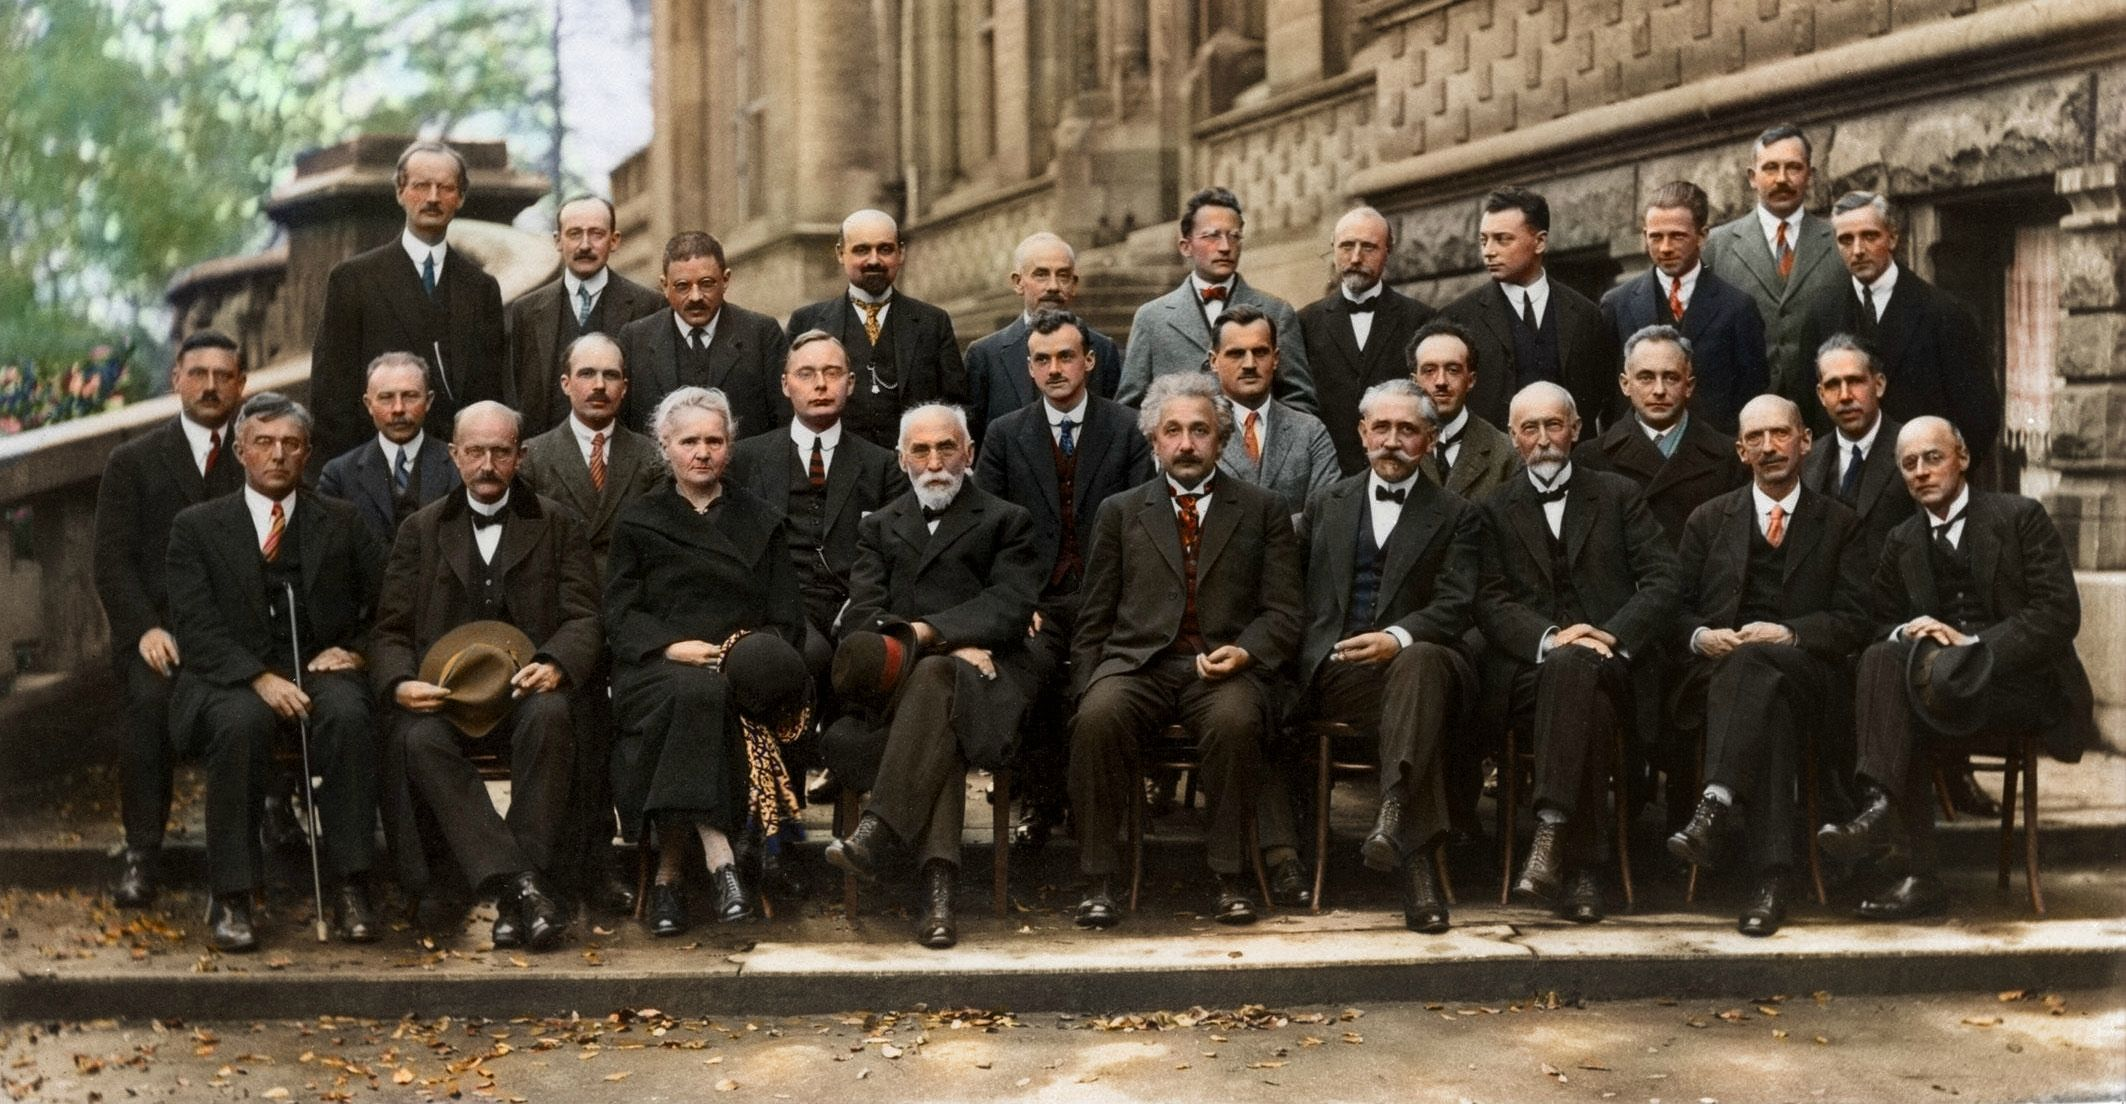
\includegraphics[width=0.8\linewidth]{solvay}
  \caption{V Сольвеевский конгресс (1927) «Электроны и фотоны»}
  \label{fig:logo}
\end{figure}

Ниже (см. табл.~\ref{tab:sampletable}) представлен вариант таблицы с
заголовком оформленным с помощью \verb"\caption".

\begin{table}
  \centering
  \caption{Пример небольшой таблицы}
  \label{tab:sampletable}
  \begin{tabular}{|c|c|c|c|c|}
    \hline
    Номер & $X$ & $Y$ & $R$ & Цвет\\
    \hline
    1 &     100  &  170 & 30 & красный\\
    2 &     100  &  90      & 60 & жёлтый\\
    3 &     230  &  250     & 50 & синий\\
    4 &     130  &  240 & 60 & зелёный\\
    5 & 300  &      130 & 30 & зелёный\\
    6 &     200  &  150     & 90 & красный\\
    \hline
  \end{tabular}
\end{table}

Для ссылки на источники необходимо использовать команду \verb"\cite".

Литература может формироваться либо с помощью программы \verb"bibtex",
либо с помощью окружения \verb"thebibliography".
При формировании списка литературы просьба использовать стандарт
ГОСТ~Р7.0.5-2008. Примеры цитирования книги~\cite{mathtensor,
  jones-fogelin:tcqd}, раздела в книге~\cite{Muller2006},
статьи~\cite{Arduengo1991, Booth1962},
материалов конференции~\cite{Hope2005}.

На все источники в списке литературы должны быть ссылки.

\section{Заключение}

Заключение является неотъемлемой частью любой работы.

Оно должно содержать краткие выводы по результатам исследования,
отражающие новизну и практическую значимость работы, предложения по
использованию ее результатов, оценку её эффективности и качества.

% \section{Ethical disclaimers}

% A disclaimer is a note of disclaimer of responsibility~\cite{kulyabov_2024_editorial_author-ethics_en}.
% For example, authors' statements about conflicts of interest, author contributions, acknowledgements, etc.

% Authors should not prepare these disclaimers as a numbered or unnumbered
% \mintinline{latex}{\section}%
% ; please use the special environments instead.

% \subsection{Author contributions}

% The Committee on Publication Ethics (COPE) draws attention to the problem of authorship \cite{cope_book_authorship_en}.
% The CRediT system (\url{https://credit.niso.org/}) is proposed to formalize author roles.
% The CRediT (Contributor Roles Taxonomy) offers 14 possible author roles \cite{holcombe_2019_contributorship-not-authorship_en}.
% This is not really a taxonomy, but a faceted classification. Author roles are not always independent in themselves.

% The following statements should be used \emph{Conceptualization, X.X. and Y.Y.; methodology, X.X.; software, X.X.; validation, X.X., Y.Y. and Z.Z.; formal analysis, X.X.; investigation, X.X.; resources, X.X.; data curation, X.X.; writing---original draft preparation, X.X.; writing---review and editing, X.X.; visualization, X.X.; supervision, X.X.; project administration, X.X.; funding acquisition, Y.Y.}
% Please add at the end of the statement:
% \emph{All authors have read and agreed to the published version of the manuscript.}

% This section has a special environment:
% \begin{minted}{latex}
% \begin{authorcontributions}
% …
% \end{authorcontributions}
% \end{minted}

% \subsection{Funding}

% Disclaimer \emph{funding} refers primarily to external funding if the research was externally initiated.
% If the research is entirely the initiative of the author's team, it is better to indicate gratitude for partial funding of some of the stages of the research in the \emph{Acknowledgments} section.
% The fact that the author's team has received external funding should be recorded in the disclaimer as a matter of course.
% When mentioning the sponsor, its exact data (name of the organization, grant number, etc.) and the country of its location should be specified (for example \emph{This research was funded by NAME OF FUNDER grant number XXX}).
% If there is any support, it is recommended to clarify in the \emph{Conflicts of interest} section at which stages of the research and how the support was used.
% If there is no external funding, it is written: \emph{This research received no external funding}.
% If it is impossible to obtain information from the authors about the source of funding, then write: \emph{Not specified}.

% This section has a special environment:
% \begin{minted}{latex}
% \begin{funding}
% …
% \end{funding}
% \end{minted}

% \subsection{Data availability statement}

% Data are particularly important in reproducible researches.
% The data availability statement tells the reader where the research data related to the article are located and under what conditions the data can be accessed.
% References to the dataset are also provided.

% If no new data is created or analyzed, please write:
% \emph{No new data were created or analyzed in this study. Data sharing is not applicable.}

% This section has a special environment:
% \begin{minted}{latex}
% \begin{dataavailability}
% …
% \end{dataavailability}
% \end{minted}

% \subsection{Conflicts of interest}

% This disclaimer must be included.

% Conflicts of interest can comment on various aspects, but usually the author's past or current employment is indicated.
% Grants (especially from for-profit companies) received not only by the author but also by the organization for which he or she works are indicated.
% If the author is associated with a sponsor, it is indicated where the research was conducted.

% If there is no conflict of interest, then the corresponding statement should also be included: \emph{The authors declare no conflict of interest}.

% This section has a special environment:
% \begin{minted}{latex}
% \begin{conflictsofinterest}
% …
% \end{conflictsofinterest}
% \end{minted}

% \subsection{Acknowledgments}

% Identification of funding sources and other support, and thanks to individuals and groups that assisted in the research and the preparation of the work should be included in an acknowledgment section, which is placed just before the reference section in your document.

% This section has a special environment:
% \begin{minted}{latex}
% \begin{acknowledgments}
% These are different acknowledgments.
% \end{acknowledgments}
% \end{minted}
% so that the information contained therein can be more easily collected during the article metadata extraction phase, and to ensure consistency in the spelling of the section heading.

% \section{Appendices}

% If your work needs an appendix, add it before the
% \mintinline{latex}{\end{document}}
% command at the conclusion of your source document.

% Start the appendix with the
% \mintinline{latex}{\appendix}
% command:
% \begin{minted}{latex}
% \appendix
% \end{minted}
% and note that in the appendix, sections are lettered, not numbered.

\vspace{\baselineskip}

\begin{authorcontributions}
  Концептуализация, написание --- рецензирование и редактирование: Анна Владиславовна Королькова; методология, написание --- подготовка первоначального варианта: Дмитрий Сергеевич Кулябов.
  Все авторы прочитали и согласились с опубликованной версией рукописи.
\end{authorcontributions}

\begin{funding}
  Данное исследование не получало внешнего финансирования.
\end{funding}

\begin{dataavailability}
  В ходе исследования не было создано и проанализировано никаких новых данных. Совместное использование данных неприменимо.
\end{dataavailability}

\begin{conflictsofinterest}
  Авторы заявляют об отсутствии конфликта интересов.
\end{conflictsofinterest}

\begin{acknowledgments}
  Мы благодарим организаторов конференции за предоставленную возможность создать этот шаблон.
\end{acknowledgments}

\begin{aideclaration}
  Авторы не использовали никаких инструментов генеративного искусственного интеллекта.
\end{aideclaration}


%%
%% Define the bibliography file to be used
\printbibliography

%%
%% If your work has an appendix, this is the place to put it.
\appendix

\section{Локальная компиляция}

Чтобы скомпилировать проект, выполните команду:
\begin{minted}{shell}
latexmk
\end{minted}

После компиляции очистите проект:
\begin{minted}{shell}
latexmk -C
\end{minted}


\section{Онлайн-ресурсы}


\begin{itemize}
\item GitHub: \url{https://github.com/yamadharma/ittmm-author-template}.
\item GitVerse: \url{https://gitverse.ru/dharma/ittmm-author-template}.
\end{itemize}

\end{document}

%%% Local Variables:
%%% mode: LaTeX
%%% TeX-master: t
%%% End:
